\documentclass[twocolumn,preprintnumbers,amsmath,amssymb,longbibliography]{revtex4-1}

\usepackage{graphicx}% Include figure files
\usepackage{dcolumn}% Align table columns on decimal point
\usepackage{bm}% bold math
\usepackage{float}
\usepackage{siunitx}

% Set one inch margins all around
\setlength\textwidth{6.5in}
\setlength\oddsidemargin{0in}
\setlength\evensidemargin{0in}

\setlength\textheight{9in}
\setlength\topmargin{-0.25in}
\setlength\headheight{0in}

\begin{document}

\title{Measurement of the Gravitational Acceleration}% Force line breaks with \\

\author{Aether Zhou}
\affiliation{%
Department of Physics, University of California, Santa Barbara, CA 93106
}%

\date{\today}% It is always \today, today

\begin{abstract}
    For a simple pendulum under small angle oscillation, its period is proportional to the square-root of the string length. This paper will introduce a simple pendulum experiment conducted recently and provide a brief examination of the square-root proportional relation. Also, the experiment provide a simple way to measure the gravitational acceleration on the Earth based on the known relation between pendulum period and string length. 
\end{abstract}

\maketitle

\section{Introduction}
\label{intro}
For an oscillating simple pendulum in Fig.~\ref{sp}, the system's motion can be described by  
\begin{eqnarray}
\ddot{\theta}=-\frac{g}{l}\sin{\theta} \, .
\end{eqnarray}
For small angle oscillation, we can approximate its motion linearly
\begin{eqnarray}
\ddot{\theta}=-\frac{g}{l}\theta \, ,
\end{eqnarray}
and the period is given by
\begin{eqnarray}
T=2\pi\sqrt{\frac{l}{g}} \label{period}\, .
\end{eqnarray}
This paper will use a simple pendulum experiment to check the relationship between the period and the string length and roughly measure the gravitational acceleration $g$.
\begin{figure}[H]
\centering
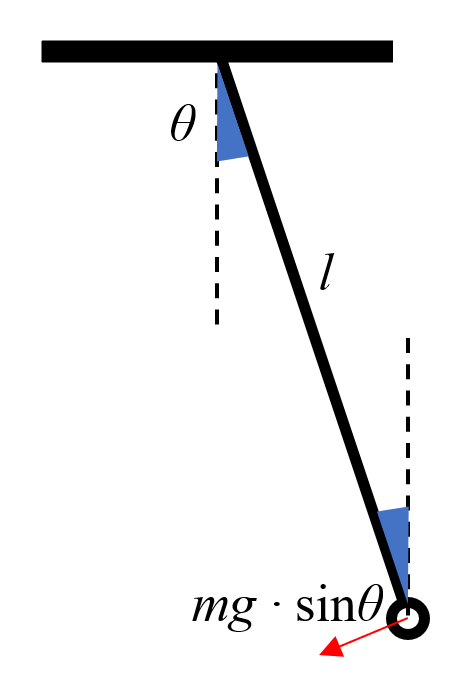
\includegraphics[width=4cm]{simplePendulum.png}
\caption{\label{sp} A simple pendulum.} 
\end{figure}

\section{Experimental Methods}
As shown in Fig.~\ref{app}, The apparatus used contains a string fixer, a desk, a protractor, a string and a weight. The string fixer is built with several books providing enough friction to fix the string. The protractor is used to determine the releasing angle, with minimum scale of one degree. The effective length of the string is measured with a ruler to the uncertainty of one centimeter. And the weight is composed with a light plastic bag and several metal coins.
\begin{figure}[H]
\centering
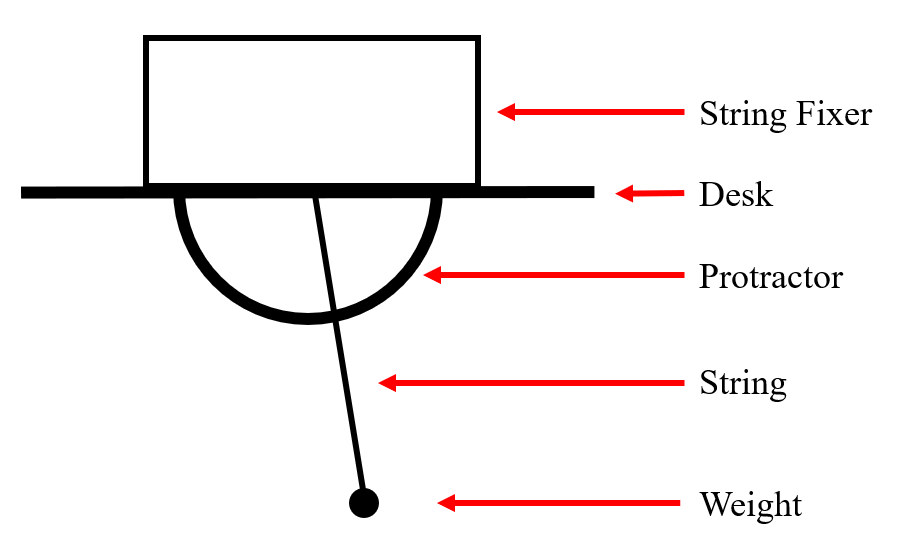
\includegraphics[width=7cm]{apparatus.png}
\caption{\label{app} Apparatus structure.} 
\end{figure}
Three possible variables relating to the period was considered: weight, releasing angle, and string length. For each of the variables, seven cases were considered, and each case is repeated six times so that a statistically significant result could been reached. And a stop watch is used to record the time from releasing weight to the end of the fifth round of travelling, so the measured period for each trail is the measured time divided by five.

\section{Results}
To check dependence of period on mass, amplitude and length, different weights are divided into seven sets from twenty to eighty coins. Similar for amplitude and length, they vary from three to twenty first degrees and from ten to seventy centimeters. 
The periods of the simple pendulum under different releasing angles or different loaded weights do not have statistically significant differences.
\begin{figure}[H]
\centering
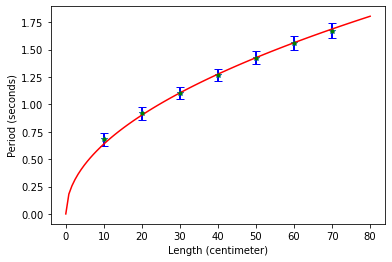
\includegraphics[width=7cm]{TvL.png}
\caption{\label{tvl} Period-length graph.} 
\end{figure}
By using the $scipy.optimize.curve\_fit$ method in python, which is a version of least square fitting, we fit the period-length data with the relation equation \eqref{period}. And the fitted value for gravitational acceleration is about $9.71\, \si{.m.s^{-2}}$. 

\section{Analysis} 
For the period-length relation, the string length are measured with uncertainty of $\pm 1$ centimeter, and the periods are measured with uncertainty of $\pm 0.1$ seconds. The uncertainty in periods measurement are contributed by human reaction time, which is taken as a random number around $0.1$ seconds. Hence, the uncertainty for the fitted gravitational acceleration 
\begin{table}[H]
\caption{\label{table}Summary of the systematic uncertainties}
\begin{ruledtabular}
\begin{tabular}{ll}
Source&Uncertainty\\
\hline
measuring length with ruler & $0.05$ \\
extension of the string & $0.005$ \\
stopwatch & $0.01$ \\
human reaction time & $0.04$ \\
\hline
Total&$0.105$\\
\end{tabular}
\end{ruledtabular}
\end{table}
Hence, the systematic uncertainty of the measured gravitational acceleration is about $10.5$ percent, and $9.8 \si{.m.s^{-2}}$ falls in the region of $(9.71\pm 1.02) \si{.m.s^{-2}}$.
\section{Conclusions}
In conclusion, from this simple pendulum experiment, we checked the accuracy of the square root proportional relation between period and string length of a simple pendulum. We also shown that the weight and amplitude are irrelevant to the period. \ref{intro}

\begin{acknowledgments}
Thanks to Andrew Jayich for the guidance of the experiment and editing this report. 
\end{acknowledgments}

\appendix

\section{Extra Text}



\bibliography{references}% Produces the bibliography via BibTeX.

\end{document}
%
% ****** End of file apssamp.tex ******
